\documentclass[leqno]{article}
\usepackage[utf8]{inputenc}
\usepackage{enumitem}
\usepackage{tikz}
\usepackage[parfill]{parskip}
\usepackage{mathtools}
\usepackage{amsmath}
\usepackage{amssymb}

\title{Computationele logica}
\author{
    Kamans, Jim\\
    \texttt{10302905}
    \and
    Roosingh, Sander\\
    \texttt{11983957}
    \and
    Schenk, Stefan\\
    \texttt{11881798}
}
\date{December 2017}

\begin{document}

\maketitle

%%%%%%%%%%%%%%%%%%%%%%%%%%%%%%%%%%%%%%%%%%%%%%%%%%%%%%%%%%%%%%%%%%%%%%%%%%%%%%%
%% Exercise 1 %%
%%%%%%%%%%%%%%%%%%%%%%%%%%%%%%%%%%%%%%%%%%%%%%%%%%%%%%%%%%%%%%%%%%%%%%%%%%%%%%%
\section*{Exercise 1}
A robot is in a war zone. It doesn’t know its location, but all it cares is
whether or not there is a mine in front (m), and whether or not there is an
enemy approaching (e).

\begin{enumerate}
  \item \textit{Represent the robots’s belief-revision structure using a
  single-agent plausibility model, with four possible states, using the atomic
  sentences m for “there is a mine in front of the robot”, and e for “an enemy
  is approaching”.}

  \begin{center}
  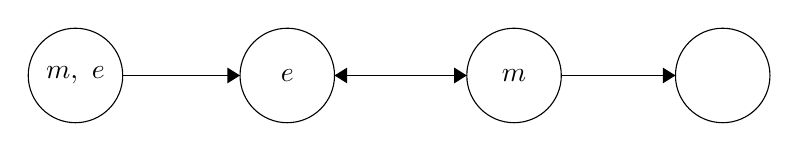
\begin{tikzpicture}[scale=0.2]
  \tikzstyle{every node}+=[inner sep=0pt]
  \draw [black] (35.95,-14.6) circle (3);
  \draw (35.95,-14.6) node {$e$};
  \draw [black] (50.35,-14.6) circle (3);
  \draw (50.35,-14.6) node {$m$};
  \draw [black] (63.6,-14.6) circle (3);
  \draw [black] (22.5,-14.6) circle (3);
  \draw (22.5,-14.6) node {$m,\mbox{ }e$};
  \draw [black] (38.95,-14.6) -- (47.35,-14.6);
  \fill [black] (47.35,-14.6) -- (46.55,-14.1) -- (46.55,-15.1);
  \draw [black] (47.35,-14.6) -- (38.95,-14.6);
  \fill [black] (38.95,-14.6) -- (39.75,-15.1) -- (39.75,-14.1);
  \draw [black] (25.5,-14.6) -- (32.95,-14.6);
  \fill [black] (32.95,-14.6) -- (32.15,-14.1) -- (32.15,-15.1);
  \draw [black] (53.35,-14.6) -- (60.6,-14.6);
  \fill [black] (60.6,-14.6) -- (59.8,-14.1) -- (59.8,-15.1);
  \end{tikzpicture}
  \end{center}

  \item \textit{Suppose now that the robot’s sensors indicate some vibrations.}

  \begin{center}
  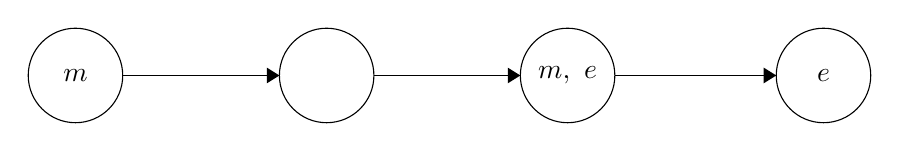
\begin{tikzpicture}[scale=0.2]
  \tikzstyle{every node}+=[inner sep=0pt]
  \draw [black] (65.45,-11.7) circle (3);
  \draw (65.45,-11.7) node {$e$};
  \draw [black] (17.95,-11.7) circle (3);
  \draw (17.95,-11.7) node {$m$};
  \draw [black] (33.9,-11.7) circle (3);
  \draw [black] (49.2,-11.7) circle (3);
  \draw (49.2,-11.7) node {$m,\mbox{ }e$};
  \draw [black] (20.95,-11.7) -- (30.9,-11.7);
  \fill [black] (30.9,-11.7) -- (30.1,-11.2) -- (30.1,-12.2);
  \draw [black] (36.9,-11.7) -- (46.2,-11.7);
  \fill [black] (46.2,-11.7) -- (45.4,-11.2) -- (45.4,-12.2);
  \draw [black] (52.2,-11.7) -- (62.45,-11.7);
  \fill [black] (62.45,-11.7) -- (61.65,-11.2) -- (61.65,-12.2);
  \end{tikzpicture}
  \end{center}

  \item \textit{Immediately after the event in the previous part, the robot’s metal detector indicates the presence of a mine}

  \begin{center}
  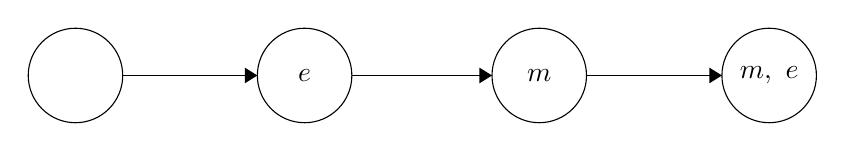
\begin{tikzpicture}[scale=0.2]
  \tikzstyle{every node}+=[inner sep=0pt]
  \draw [black] (35.95,-22.9) circle (3);
  \draw (35.95,-22.9) node {$e$};
  \draw [black] (50.85,-22.9) circle (3);
  \draw (50.85,-22.9) node {$m$};
  \draw [black] (21.4,-22.9) circle (3);
  \draw [black] (65.45,-22.9) circle (3);
  \draw (65.45,-22.9) node {$m,\mbox{ }e$};
  \draw [black] (24.4,-22.9) -- (32.95,-22.9);
  \fill [black] (32.95,-22.9) -- (32.15,-22.4) -- (32.15,-23.4);
  \draw [black] (38.95,-22.9) -- (47.85,-22.9);
  \fill [black] (47.85,-22.9) -- (47.05,-22.4) -- (47.05,-23.4);
  \draw [black] (53.85,-22.9) -- (62.45,-22.9);
  \fill [black] (62.45,-22.9) -- (61.65,-22.4) -- (61.65,-23.4);
  \end{tikzpicture}
  \end{center}

  \item \textit{}

\end{enumerate}

%%%%%%%%%%%%%%%%%%%%%%%%%%%%%%%%%%%%%%%%%%%%%%%%%%%%%%%%%%%%%%%%%%%%%%%%%%%%%%%
%% Exercise 2 %%
%%%%%%%%%%%%%%%%%%%%%%%%%%%%%%%%%%%%%%%%%%%%%%%%%%%%%%%%%%%%%%%%%%%%%%%%%%%%%%%
\section*{Exercise 2}
\begin{enumerate}

	\item

	\item

	\item

	\item

	\item

\end{enumerate}

\end{document}
